\subsection{Constrained Spreading Activation}
One of the leading features of SA technique is its flexibility to fit to 
the resolution of different kind of problems. From the configuration point of view
some constraints presented in~\cite{Cohen1987} have been customized to improve
the expected outcomes of the execution according to the domain problem. 

\begin{description}

\item [Distance:] nodes far from an activated node should be penalized due to
the number of needed steps to reach and activate them.

\item [Path:] the activation path is built by the activation process from a node
to other and this process can be guided according to the weights of relations (edges). 

\item [Multiple outputs (Fan-Out):] ``highly connected'' nodes can 
guide to a misleading situation in which activated and spread nodes are not representative, these nodes
should be skipped or penalized by the algorithm.

\item [Threshold activation:] a node $n_i$ will be spread $iif$ its activation
value, $I_i$, is greater than a threshold activation constant $\jmath$.

\end{description}

The aforementioned theoretical model is an excellent start point to design
a framework for \textit{SA} but from the domain expert point of view some configuration
requirements to apply this technique to ontologies are missing. 
That is why a set of extensions are proposed to deal with the specific features 
of RDF graphs and ontologies.

\begin{description}

\item[Context of activation $\mathbb{D}_{com}$:] the framework is able to manage some ontologies
at the same time and concepts can be defined in different ontologies identified
by a context URI (or namespace). The double process of activation and spreading will only be performed in the
set of active contexts $\mathbb{D}_{com}$.


\begin{definition}
Let $\mathbb{D}_{com}$ an active domain, if a concept $c_i$ is activated o
spread then $c_{i} \in \mathbb{D}_{com}$.
\end{definition}

\item[Minimum activation value $N_{\min}$ :] only concepts with an activation
value $N_k$ greater than $N_{\min}$ will be spread. This constraint comes from
the theoretical model of \textit{SA}.

\item[Maximum number of spread concepts $\mathbb{M}$ :] the process of
activation and spreading will be performed, at the most, until $\mathbb{M}$ concepts
had been spread.

\item[Minimum number of spread concepts $\mathbb{M_{\min}}$ :] the process of
activation and spreading will be performed, at least, $\mathbb{M_{\min}}$ concepts had
been spread.

\item[Time of activation $t$:] the process of activation and spreading
will be performed, at the most, during $t$ units of time.

\item[Output Degradation $O_j$:] one of the keypoints to improve and customize
the algorithm is to define a function $h$ that penalizes the output value $O_j$
of a concept $c_j$.

\begin{enumerate}

\item Generic customization: $h$ calculates the output of a concept $c_j$
according to its degradation level.

\begin{equation}
O_j = h(I_j)
\end{equation}

Basic case: if $h_0 = id$, the output value $O_j$ takes the level of the
activated concept $c_j$ as its value.

\begin{equation}
O_j = h_0(I_j) = I_j
\end{equation}


\item Customization using {\bf distance}: $h_1$ calculates the level activation
of the concept $c_j$  according to the distance from the initial concept $c_l
\in \Phi$\footnote{Set of initial concepts.} to the node that has activated it. The
activation value should decrease if the distance from $\Phi$ grows thus
the algorithm follows a path from $c_l$ to $c_j$: $I_l > I_j$.


The function $h_1$ penalizes the output of concepts (decreasing their rank)
far from the ``activation core'' and rewards closed concepts. Thus, let $d_j$,
where $d_j = min\{d_{lj}:\forall n_l \in \Phi\}$:


\begin{equation}
 O_j = h_1(I_j,d_j)= \frac{I_j} {d_j}
\end{equation}

\item Customization using {\bf beats}: the function $h_2$ calculates the
degradation of the concept using the number of iterations $k$:

\begin{equation}
 O_j = h_2(I_j,k) = (1+\frac{I_j}{k})\exp(-\frac{I_j}{k}).
\end{equation}

\end{enumerate}

\end{description}

\subsection{Specification of the SA technique}\label{impl-sa}
The entry point to SA technique is the set of initial concepts that will generate 
a new set of the most relevant concepts. Ontologies based on the RDF graph model are a graph where each node $n_i$ represents a concept
$c_i$ and the edge $\omega_{ji}$ is the semantic relation between $c_j$ y $c_i$.
The final result of the algorithm is a set of sorted pairs $(n_i, I_i)$
that builds the set of output concepts, where $n_i\approx c_i$ and $I_i\approx w_i$ (the
relevance of the concept). The implementation of \textit{SA}, see Algorithm~\ref{alg:as}, comprises of two sets of concepts that
store information about the state of the algorithm: 1) $\mathbb{D}_{com}$ are all the concepts in the semantic network 
and 2) $\Phi$ is the set of initial activated concepts, $c_j^k$  is the spreading concept 
at the $k$-th iteration (from which other concepts are activated).

Set $\mathcal{A}$: queue of {\bf activated} concepts (candidates to be
spread).

\begin{align}
 \mathcal{A}^0 &=\Phi \\
 \mathcal{A}^k &=(\mathcal{A}^{k-1} \cup \{c_i: {\forall c_i /  \omega_{ji}^k
>0}\})-{ \{\mathcal{G}^k}\}
\end{align}

Set $\mathcal{G}$: set of {\bf spread} concepts.

\begin{align}
 \mathcal{G}^0 &=\emptyset \\
 \mathcal{G}^k &= \mathcal{G}^{k-1} \cup \{c_j^k\}
\end{align}

Finally, the calculus of the activation value of a concept $c_i$
at iteration $k$, indicated by $I^k_i$, is defined. At $0$ iteration the
activation value $c_i$ is calculated as follows:
\begin{equation}
I^0_i=\begin{cases}%
  1 & \text{if $c_i \in \Phi$} \\%
  0 & \text{if $c_i \notin \Phi$} \\%
 \end{cases}
\end{equation}

at $k$ iteration, the activation value of $c_i$ from element
$c_j^{k}$ to $c_i$ is calculated as follows:

\begin{equation}
I^k_i=\begin{cases}%
  I^{k-1}_i & \text{if } \omega_{ji}^k = 0 \\%
  I^{k-1}_i + \omega_{ji}^k I^{k-1}_j  & \text{if }  \omega_{ji}^k > 0  \\%
 \end{cases}
\end{equation}

\begin{algorithm}
\caption{\textit{Pseudocode of Spreading Activation}}
\label{alg:as}
\begin{algorithmic}
  \REQUIRE $\Phi \neq \emptyset$  
  \ENSURE $\mathcal{G} \neq \emptyset$
  \STATE $\mathcal{A} \leftarrow \Phi$
  \STATE $\mathcal{G} \leftarrow \emptyset$
  \WHILE{$\mathcal{A} \neq \emptyset$ AND $card(\mathcal{G}) <
\mathcal{G}_{\min}$ AND $N_k \ge N_{\min}$}
	\STATE $n_k \leftarrow  extract(\mathcal{A})$
	\STATE $\mathcal{G} \leftarrow \{n_k\} \cup \mathcal{G}$	  	
	  \FORALL{$n_i / w_{ki} > 0$}	  	
	  	\STATE $N_i \leftarrow N_i + w_{ki}N_k$	
		\STATE $\mathcal{A} \leftarrow (\{n_i\} \cup \mathcal{A}) -
\mathcal{G}$		
	    \ENDFOR
  \ENDWHILE
 \RETURN $\mathcal{G}$
\end{algorithmic}
\end{algorithm}\label{alg:as}

\subsection{Improving Spreading Activation}\label{improve:sa}
Some improvements in the calculus of the activation value of a
concept have been introduced in order to get a more complete and accurate technique. 
If some paths of activation converge to the same node and the source nodes are different then this node should be 
relevant and a reward is applied to the nodes presented in these paths. 

\begin{definition}
Let $p_i$ the number of paths that start and finish in different nodes of
$\Phi$\footnote{The reward is not applied to nodes in  $\Phi$.} and they go
through the node $c_i$ and they only contain nodes belonging to $\mathcal{G}$.
This improvement assigns a new value to the activation value of each node $c_i$
indicated by $I^*_i$ and it is calculated by means of the function $g$:
\end{definition}

\begin{equation}
I^*_i = g(I_i,p_i)
\end{equation}

In this case, a relaxed reward function has been chosen, Eq.~\ref{f:recompensa},
and, it is applied in the \textit{Postadjustment} stage, thus the
original semantics and behavior of \textit{SA} algorithm remains. 

\begin{equation}\label{f:recompensa}
g(x,y) = x (\log(y+1)+1)
\end{equation}

$x$ is the reward constant, it can be defined according to the context and $y$
is the number of times that a concept $c_i$ must be rewarded.

% \begin{figure}[h]
%  \centering
%     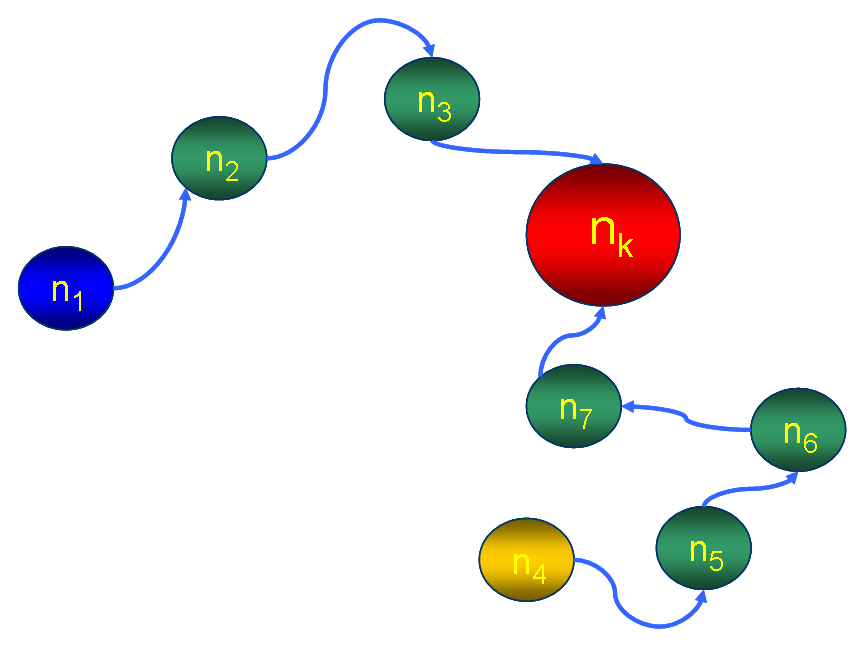
\includegraphics[width=6cm]{images/prize-sa}
%     \caption{Paths and rewards in \textit{Spreading Activation}}
%  \label{fig:prize-sa}
% \end{figure}
\subsection{Refining Spreading Activation}
The whole configuration of the algorithm can be made by default but a customization
to a particular domain should be carried out by a domain expert taking into account the
specific issues of that domain and considering it as a new stage of 
the ontology o graph modeling process. Since \textit{SA} uses weights in relations  to calculate the activation
value of the concepts, different ``patterns'' have been identified to manage the direction 
of the spreading process: 1) Ascending seeks for the activation of concepts more generic than
the current (``superclass''); 2) Descending seeks for the activation of concepts more specific than
the current (``subclass''); 3) Nominal seeks for the activation of instances instead of concepts (``instance of'')
and 4) Crossing  seeks for the activation of concepts and instances connected through a certain relation $\mathcal{R}$.
These control patterns can be put together in order to fit as much as possible the focus and 
direction of the double process of activation and spreading.

\subsection{Design and implementation of ONTOSPREAD}
ONTOSPREAD framework\footnote{\url{http://code.google.com/p/ontospread/}}, see Fig.~\ref{fig:diagramas/general}
 is addressed by an open and extensible design applying best practices on software design and development like design patterns and refactoring. 
The \textit{Player} class handles the execution of the algorithm in a  stepwise way. It is 
an application of the \textit{Iterator} design pattern to perform the activation and spreading processes. The state of 
the algorithm is captured in a separate class (\textit{OntoSpreadState}) that makes possible to serialize the 
current state and back to a previous one. On the other hand, the \textit{SA} process comprises of three sub-processes 
(see Sect.~\ref{background}): \textit{OntoSpreadPreAdjustment}; \textit{OntoSpreadRun}; and \textit{OntoSpreadPostAdjustment}. Moreover, 
the process carries on the information about the knowledge base using the DAO pattern thus the 
framework is independent from the modeling language of the semantic network (RDF-based vocabularies and OWL are now supported).

\begin{figure}[htb]
\centering
  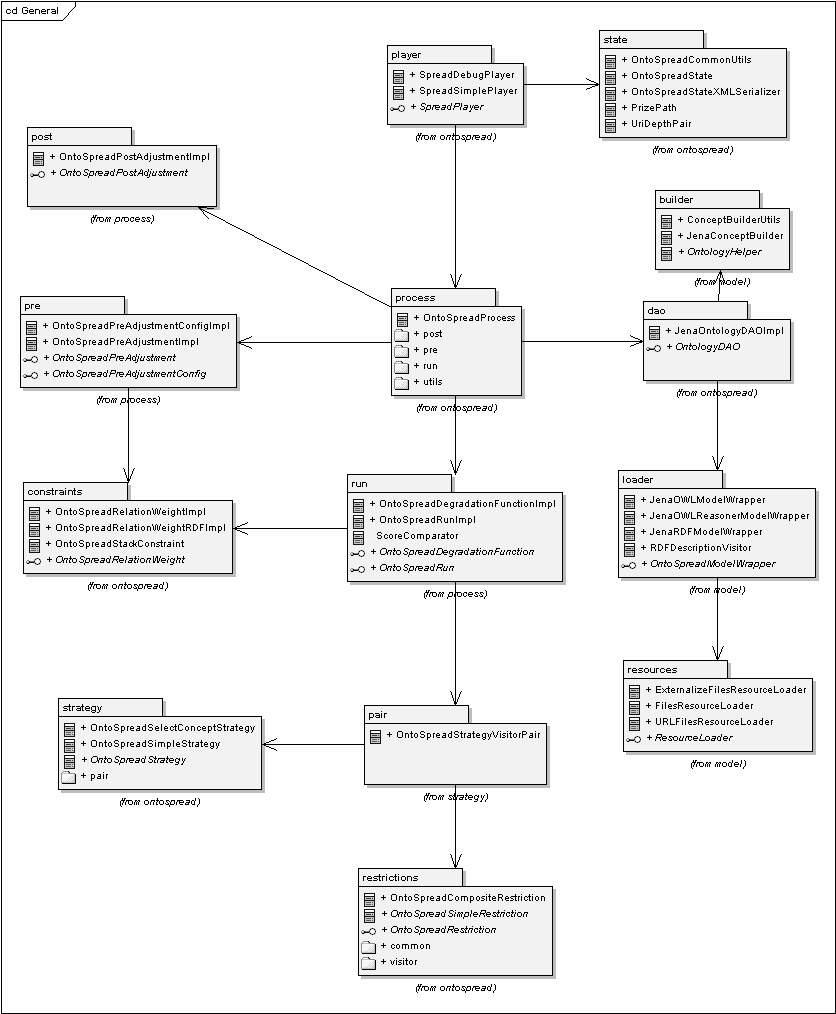
\includegraphics[width=8cm]{images/general}
\caption{ONTOSPREAD Overview Diagram.}
\label{fig:diagramas/general}
\end{figure}

The keypoint to design the algorithm lies in how and where
the information will be available at different iterations. Secondly, an unique entry point
to the state of the algorithm should be available trying to avoid
illegal accesses. This object (\textit{OntoSpreadState}) stores the next information: \begin{inparaenum}\item Spread
concepts. \item Active concepts. \item Paths of activation. \item Concept to be
spread. \item Generic swap area (to share information among iterations). \end{inparaenum}
Moreover, the extensibility and flexibility of the algorithm is subjected to a good design
of the restrictions and their evaluation process. The next features and design patterns 
are used to design and implement the model of restrictions of SA:
\begin{itemize}
  \item Any restriction can be considered as a simple restriction and can be
evaluated to a boolean value.
  \item Conditions or actions in the algorithm can be comprised of several
restrictions.
  \item The extension points of the algorithm, included through a
\textit{Template Method} design pattern, are strategies to carry out an specific
action. Each strategy can be subjected to one or more restrictions.
\item Each restriction can be simple or comprised of others. \textit{Composite} pattern.
  \item Each action is an strategy. \textit{Strategy} pattern.
  \item A strategy implies one restriction (or a set of them) thus the strategy
is a client of the \textit{Composite} of restrictions.
  \item The evaluation of the restrictions to get their value (boolean) is
carried out through a \textit{Visitor} pattern that fits perfectly to evaluate and walk in
composite objects. It consists on: apply the strategy that modifies the state
of the algorithm and assert this change of state by means of the restrictions applied
to this strategy.
\end{itemize}

% \subsection{Development of ONTOSPREAD API and Supporting Tools}
% The development of the API has been performed using Semantic Web and Java technologies
% like: Jena\footnote{\url{http://jena.sf.net}} API, JAXB\footnote{\url{
% http://java.sun.com/developer/technicalArticles/WebServices/jaxb/}}, 
% Maven\footnote{\url{http://maven.apache.org}} o
% Spring\footnote{\url{http://www.springframework.org/}}. Besides two tools are provided to test and debug different configurations
% of the algorithm:
% 
% \begin{itemize}
%  \item [ONTOSPREAD-TEST] It is a tool for the automatic execution and reporting
% of batch tests. It provides an user-oriented framework to configure, combine and load several
% configurations (e.g. restrictions, weights, initial concepts, etc.) for \textit{SA} and get results. A XML
% vocabulary using XML-Schema and the \textit{Extensible Content Model} XML design
% pattern has been defined to build the configuration of the \textit{SA} process.
%  The designing of this vocabulary is oriented to be used with JAXB, this technology enables us 
% automatically the processes of marshalling and unmarshalling Java classes providing an easy way to configure, 
% load and serialize the different configurations and results. 
% 
% \item [ONTOSPREAD Inspector.] It is a graphical debugger of \textit{SA} algorithm 
% using the graph library JpowerGraph\footnote{\url{http://jpowergraph.sf.net}} and
% the SWT\footnote{\url{http://www.eclipse.org/swt/}} toolkit. It enables to configure, load, 
%  run (one step or stepwise) and view the evolution of the semantic network 
%  with the concepts (activated, spread, weights, relations, etc.).
% \end{itemize}
% 
% Finally, a set of source code metrics using Eclipse\footnote{\url{http://www.eclipse.org}} and the 
% metrics plugin\footnote{\url{http://metrics.sf.net/}} have been extracted to demonstrate and measure its 
% quality. Table\ref{tabla:metricas-valores} presents these metrics that measures cohesion and coupling 
% of the software.
%    \begin{longtable}{|p{1cm}|p{4cm}|p{1cm}|p{1cm}|p{1cm}|p{1cm}|p{1.5cm}|}
%         
%         \caption{Source Code Metrics} \label{tabla:metricas-valores}\\
%         \hline
%         \multicolumn{7}{|c|}{\textbf{Source Code Metrics}}\\
%         \hline\subsection{Development of ONTOSPREAD API and Supporting Tools}
% The development of the API has been performed using Semantic Web and Java technologies
% like: Jena\footnote{\url{http://jena.sf.net}} API, JAXB\footnote{\url{
% http://java.sun.com/developer/technicalArticles/WebServices/jaxb/}}, 
% Maven\footnote{\url{http://maven.apache.org}} o
% Spring\footnote{\url{http://www.springframework.org/}}. Besides two tools are provided to test and debug different configurations
% of the algorithm:
% 
% \begin{itemize}
%  \item [ONTOSPREAD-TEST] It is a tool for the automatic execution and reporting
% of batch tests. It provides an user-oriented framework to configure, combine and load several
% configurations (e.g. restrictions, weights, initial concepts, etc.) for \textit{SA} and get results. A XML
% vocabulary using XML-Schema and the \textit{Extensible Content Model} XML design
% pattern has been defined to build the configuration of the \textit{SA} process.
%  The designing of this vocabulary is oriented to be used with JAXB, this technology enables us 
% automatically the processes of marshalling and unmarshalling Java classes providing an easy way to configure, 
% load and serialize the different configurations and results. 
% 
% \item [ONTOSPREAD Inspector.] It is a graphical debugger of \textit{SA} algorithm 
% using the graph library JpowerGraph\footnote{\url{http://jpowergraph.sf.net}} and
% the SWT\footnote{\url{http://www.eclipse.org/swt/}} toolkit. It enables to configure, load, 
%  run (one step or stepwise) and view the evolution of the semantic network 
%  with the concepts (activated, spread, weights, relations, etc.).
% \end{itemize}
% 
% Finally, a set of source code metrics using Eclipse\footnote{\url{http://www.eclipse.org}} and the 
% metrics plugin\footnote{\url{http://metrics.sf.net/}} have been extracted to demonstrate and measure its 
% quality. Table\ref{tabla:metricas-valores} presents these metrics that measures cohesion and coupling 
% of the software.
%    \begin{longtable}{|p{1cm}|p{4cm}|p{1cm}|p{1cm}|p{1cm}|p{1cm}|p{1.5cm}|}
%         
%         \caption{Source Code Metrics} \label{tabla:metricas-valores}\\
%         \hline
%         \multicolumn{7}{|c|}{\textbf{Source Code Metrics}}\\
%         \hline
%         \textit{ID} &  \textit{Def.} &  \textit{Total} &  \textit{Avg.}& 
% \textit{Std. Dev.} & \textit{Max}& \textit{Scope} \\ \hline
%         \endfirsthead
%         \caption[]{Source Code Metrics (continue)}\\
%         \hline
%         \multicolumn{7}{|c|}{\textbf{Source Code Metrics}}\\
%         \hline
%         \textit{ID} & \textit{Def} & \textit{Total} &  \textit{Avg.}& 
% \textit{Std.
%         Dev.} & \textit{Max}& \textit{Scope} \\ \hline
%         \endhead
%         \hline
%         \multicolumn{7}{|c|}{Continue $\ldots$}\\
%         \hline
%         \endfoot
%         \hline
%         \endlastfoot
% 		TLOC&Total Lines of Code.&5272&&&& \\ \hline
%     		CA&Afferent Coupling.&&$6.524$&$10.545$&48&Package.\\ \hline
% 		RMD&Normalized Distance, $|RMA + RMI - 1 |$.&&$0.32$&$0.347$&1&Package. \\ \hline
% 		NOM&&$0.065$&$0.296$&3&Type. \\ \hline 
% 		RMI&Instability: $CE / (CA + CE)$&&$0.567$&$0.387$&1&Package. \\ \hline
% 		%NOF&Number of Atributtes.&147&$1.256$&$2.039$&12&Type. \\ \hline
% 		%NOP&Number of Packages.&42&&&& \\ \hline
% 		%MLOC&Method Lines of Code.&2661&$4.05$&$6.179$&88&Method. \\ \hline
% 		%WMC&Weighted methods per Class.&852&$7.282$&$6.859$&42&Type. \\ \hline
% 		%NORM&Number of Overriden Methods (no ``Object'' methods).&20&$0.171$&$0.419$&2&Type. \\ \hline
% 		%NSF&Number of Static Attributes.&58&$0.496$&$0.622$&$3$&Type. \\ \hline
% 		NBD&Nested Block Depth.&&$1.204$&$0.516$&4&Method. \\ \hline
% 		%NOM&Number of Methods.&594&$5.077$&$5.297$&33&Type.\\	\hline 
% 		LCOM&Lack of Cohesion of Methods (\textit{Henderson-Sellers}).&&$0.18$&$0.289$&$0.957$&Type.\\ \hline 
% 		VG&McCabe Cyclomatic Complexity.&&$1.297$&$0.735$&6&Method. \\ \hline
% 		RMA&Abstractness.&&$0.113$&$0.186$&0.667&Package. \\ \hline
% 		%NOI&Number of Interfaces.&11&$0.262$&$0.537$&2&Package. \\ \hline
% 		CE&Efferent Coupling.&&$1.976$&$1.282$&5&Package. \\ \hline
% 		%NC&11&$0.094$&$0.539$&5&N/A&Media y máximo por tipo. \\ \hline
% 		DIT&Depth of Inheritance Tree.&&$1.607$&$0.915$&4&Type. \\ \hline
%     	 \hline
%         \end{longtable}      
% 
% All of these values are in the default range defined in the plugin thus the quality of the source code 
% with the desired feautures of \textit{high cohesion} and \textit{low coupling} are assured.
% %         \textit{ID} &  \textit{Def.} &  \textit{Total} &  \textit{Avg.}& 
% % \textit{Std. Dev.} & \textit{Max}& \textit{Scope} \\ \hline
% %         \endfirsthead
% %         \caption[]{Source Code Metrics (continue)}\\
% %         \hline
% %         \multicolumn{7}{|c|}{\textbf{Source Code Metrics}}\\
% %         \hline
% %         \textit{ID} & \textit{Def} & \textit{Total} &  \textit{Avg.}& 
% % \textit{Std.
% %         Dev.} & \textit{Max}& \textit{Scope} \\ \hline
% %         \endhead
% %         \hline
% %         \multicolumn{7}{|c|}{Continue $\ldots$}\\
% %         \hline
% %         \endfoot
% %         \hline
% %         \endlastfoot
% % 		TLOC&Total Lines of Code.&5272&&&& \\ \hline
% %     		CA&Afferent Coupling.&&$6.524$&$10.545$&48&Package.\\ \hline
% % 		RMD&Normalized Distance, $|RMA + RMI - 1 |$.&&$0.32$&$0.347$&1&Package. \\ \hline
% % 		NOM&&$0.065$&$0.296$&3&Type. \\ \hline 
% % 		RMI&Instability: $CE / (CA + CE)$&&$0.567$&$0.387$&1&Package. \\ \hline
% % 		%NOF&Number of Atributtes.&147&$1.256$&$2.039$&12&Type. \\ \hline
% % 		%NOP&Number of Packages.&42&&&& \\ \hline
% % 		%MLOC&Method Lines of Code.&2661&$4.05$&$6.179$&88&Method. \\ \hline
% % 		%WMC&Weighted methods per Class.&852&$7.282$&$6.859$&42&Type. \\ \hline
% % 		%NORM&Number of Overriden Methods (no ``Object'' methods).&20&$0.171$&$0.419$&2&Type. \\ \hline
% % 		%NSF&Number of Static Attributes.&58&$0.496$&$0.622$&$3$&Type. \\ \hline
% % 		NBD&Nested Block Depth.&&$1.204$&$0.516$&4&Method. \\ \hline
% % 		%NOM&Number of Methods.&594&$5.077$&$5.297$&33&Type.\\	\hline 
% % 		LCOM&Lack of Cohesion of Methods (\textit{Henderson-Sellers}).&&$0.18$&$0.289$&$0.957$&Type.\\ \hline 
% % 		VG&McCabe Cyclomatic Complexity.&&$1.297$&$0.735$&6&Method. \\ \hline
% % 		RMA&Abstractness.&&$0.113$&$0.186$&0.667&Package. \\ \hline
% % 		%NOI&Number of Interfaces.&11&$0.262$&$0.537$&2&Package. \\ \hline
% % 		CE&Efferent Coupling.&&$1.976$&$1.282$&5&Package. \\ \hline
% % 		%NC&11&$0.094$&$0.539$&5&N/A&Media y máximo por tipo. \\ \hline
% % 		DIT&Depth of Inheritance Tree.&&$1.607$&$0.915$&4&Type. \\ \hline
% %     	 \hline
% %         \end{longtable}      
% % 
% % All of these values are in the default range defined in the plugin thus the quality of the source code 
% % with the desired feautures of \textit{high cohesion} and \textit{low coupling} are assured.